% !TeX program = pdflatex
% -----------------------------------------------------------------------------
% APRESENTAÇÃO: AprilTag-based Trajectory Tracking for the LIMOS Robot
% -----------------------------------------------------------------------------

\documentclass[aspectratio=169, 10pt]{beamer}

% --- PACOTES ---
\usepackage[T1]{fontenc}      % Re-added for pdflatex
\usepackage[utf8]{inputenc}   % Re-added for pdflatex
\usepackage[english]{babel}
\usepackage{microtype}
\usepackage{tcolorbox}
\usepackage{booktabs}
\usepackage{qrcode}
\tcbuselibrary{skins, breakable}

% --- TIKZ ---
\usepackage{tikz}
\usetikzlibrary{calc, positioning, arrows.meta, shadows, overlay-beamer-styles, fit}

% Estilo para animações
\tikzset{
    invisible/.style={opacity=0, text opacity=0},
    visible on/.style={alt={#1{}{invisible}}},
    alt/.code args={<#1>#2#3}{\alt<#1>{\pgfkeysalso{#2}}{\pgfkeysalso{#3}}},
}

% --- FONTES (STANDARD) ---
% We use Helvet (similar to Arial) instead of fontspec/TeX Gyre
\usepackage{helvet}
\renewcommand{\familydefault}{\sfdefault}

% --- CORES ---
\definecolor{NavyBlue}{HTML}{003366}     
% ... rest of your code ...
\definecolor{NavyBlue}{HTML}{003366}     
\definecolor{CoolGray}{HTML}{5D6D7E}     
\definecolor{CleanWhite}{HTML}{FFFFFF}   
\definecolor{LightBg}{HTML}{F8F9FA}      
\definecolor{AccentBlue}{HTML}{00AEEF}   
\definecolor{AlertRed}{HTML}{C0392B}     

% --- CONFIGURAÇÃO BEAMER ---
\setbeamercolor{background canvas}{bg=CleanWhite}
\setbeamercolor{normal text}{fg=black!85}
\setbeamercolor{frametitle}{bg=CleanWhite, fg=NavyBlue}
\setbeamercolor{title}{fg=NavyBlue}

\setbeamertemplate{navigation symbols}{}
\setbeamertemplate{headline}{} 
\setbeamercovered{invisible} % Itens futuros não aparecem

% --- RODAPÉ (AUTOR + TÍTULO DO PROJETO) ---
\setbeamertemplate{footline}{%
	\leavevmode%
	\hbox{%
		% Caixa 1: Autor
		\begin{beamercolorbox}[wd=.333333\paperwidth,ht=2.25ex,dp=1ex,center]{author in head/foot}%
			\color{CoolGray}\tiny\bfseries Martins do Lago Reis; Da Silva Ramos
		\end{beamercolorbox}%
		% Caixa 2: Título
		\begin{beamercolorbox}[wd=.333333\paperwidth,ht=2.25ex,dp=1ex,center]{title in head/foot}%
			\color{NavyBlue}\tiny\bfseries AprilTag-based Trajectory Tracking – LIMOS
		\end{beamercolorbox}%
		% Caixa 3: Número da Página
		\begin{beamercolorbox}[wd=.333333\paperwidth,ht=2.25ex,dp=1ex,right]{date in head/foot}%
			\color{CoolGray}\tiny\insertframenumber{} / \inserttotalframenumber\hspace*{2ex} 
	\end{beamercolorbox}}%
	\vskip0pt%
	% Barra de Progresso
	\ifnum\inserttotalframenumber>0
	\nointerlineskip
	\makebox[\paperwidth][l]{%
		\color{gray!10}\rule{\paperwidth}{2pt}%
		\hspace{-\paperwidth}%
		\color{AccentBlue}\rule{\dimexpr\paperwidth * \insertframenumber / \inserttotalframenumber\relax}{2pt}%
	}%
	\fi
}

% --- LOGOS EM TODOS OS SLIDES (CANTO SUPERIOR DIREITO) ---
\setbeamertemplate{frametitle}{
	\vspace{0.3cm}
	\begin{tikzpicture}[remember picture,overlay]
		\node[anchor=north east] at ($(current page.north east)+(-0.4cm,-0.25cm)$) {%
			\includegraphics[height=0.7cm]{assets/logo_UCA.jpg}
		};
	\end{tikzpicture}
	\textbf{\insertframetitle} \\
	{\color{AccentBlue}\rule{1.5cm}{1.5pt}}
}

% --- CAIXAS ---
\newtcolorbox{bluebox}[1][]{
	enhanced, colback=LightBg, colframe=NavyBlue, coltitle=white,
	fonttitle=\bfseries\small, title=#1, sharp corners, boxrule=0mm,
	leftrule=1mm, rightrule=0mm, toprule=0mm, bottomrule=0mm,
	titlerule=0mm, toptitle=1mm, bottomtitle=1mm, arc=0mm
}

\newtcolorbox{alertbox}[1][]{
	enhanced, colback=white, colframe=gray!30, coltitle=NavyBlue,
	fonttitle=\bfseries, title=#1, sharp corners, boxrule=0.5pt,
	attach boxed title to top left={yshift=-2mm, xshift=2mm},
	boxed title style={colback=white, colframe=white}
}



% ==================/// START PRESENTATION ///==================///

% --- DADOS DA APRESENTAÇÃO ---
\title{AprilTag-based Trajectory Tracking for the LIMOS Robot}
\subtitle{Synthesis Project}
\author{Joao Pedro Martins do Lago Reis and Yann Kelvem da Silva Ramos}
\date{\today}

\begin{document}
	
	% -----------------------------------------------------------------------------
	\begin{frame}[plain]
		
		% --- LOGOS NO CANTO SUPERIOR DIREITO (PROPORCIONAIS) ---
		\begin{tikzpicture}[remember picture,overlay]
			\node[anchor=north east] 
			at ($(current page.north east)+(-0.8cm,-0.6cm)$)
			{
				\includegraphics[height=1.5cm]{assets/logo_UCA.jpg}
		
			};
		\end{tikzpicture}
		
		% --- TÍTULO ---
		\vspace{2cm}
		
		{\Huge\bfseries \textcolor{NavyBlue}{AprilTag-based Trajectory Tracking}}\\[0.3cm]
		{\Large\textcolor{CoolGray}{for the LIMOS Robot}}\\[1cm]
		
		% --- AUTORES ---
		{\large\textbf{Joao Pedro Martins do Lago Reis and Yann Kelvem da Silva Ramos}}\\[0.2cm]
		{\footnotesize Master's degree in artificial perception and robotics}\\[0.2cm]
		{\footnotesize \today}
		
	\end{frame}

\begin{frame}{Outline}
    \tableofcontents[hideallsubsections]
\end{frame}



% ============================================================
% SLIDE 1 — PROBLEM
% ============================================================
\section{Problem}
\begin{frame}{Problem description}
    \textbf{Problem to solve}

    \begin{itemize}[<+->]
        \item We need a robot that can \textbf{learn a path by being guided}.
        \item Later it must \textbf{drive that same path alone}.
        \item It has to work in normal indoor rooms without fuss.
    \end{itemize}
\end{frame}



% ============================================================
% SLIDE 2 — CHALLENGES
% ============================================================
\section{Challenges}
\begin{frame}{Challenges}
    \textbf{Why this is challenging}

    \begin{itemize}[<+->]
        \item \textbf{Hardcoded paths}: someone types coordinates by hand.
        \item \textbf{No flexibility}: any small change means rebuilding code.
        \item \textbf{High barrier}: only experts can tweak routes.
    \end{itemize}
\end{frame}



% ============================================================
% SLIDE 3 — CHOSEN SETUP
% ============================================================
\begin{frame}{Chosen setup}
    \begin{columns}[T]

        % Left column
        \begin{column}{0.55\textwidth}
            \textbf{Selected Platform}

            \begin{itemize}[<+->]
                \item Robot: \textbf{LIMOS} with wheels and camera.
                \item Tags: \textbf{AprilTag} to tell where the robot is.
                \item Together they keep the pose steady while we teach and repeat.
            \end{itemize}
        \end{column}

        % Right column with animated images
        \begin{column}{0.4\textwidth}
            \centering
            \begin{overlayarea}{\textwidth}{0.55\textheight}
                % Show robot with first bullet
                \only<1>{
                    \includegraphics[width=\textwidth]{assets/limo.jpeg}

                    {\tiny \textit{Fig. 1 — LIMOS mobile robot}}
                }

                % Swap to AprilTag as soon as it is mentioned
                \only<2>{
                    \includegraphics[width=0.8\textwidth]{assets/tag_36h11.png}
                    
                    {\tiny \textit{Fig. 2 — AprilTag visual marker}}
                }

                % Keep both visible from the third point onward
                \only<3->{
                    \begin{minipage}{0.48\textwidth}
                        \includegraphics[width=\textwidth]{assets/limo.jpeg}
                    \end{minipage}
                    \hfill
                    \begin{minipage}{0.48\textwidth}
                        \includegraphics[width=\textwidth]{assets/tag_36h11.png}
                    \end{minipage}
                    
                    {\tiny \textit{Fig. 1 — LIMOS robot} \hfill \textit{Fig. 2 — AprilTag marker}}
                }
            \end{overlayarea}

        \end{column}

    \end{columns}
\end{frame}


% ============================================================
% SLIDE 4 — PROJECT GOAL
% ============================================================
\section{Project goal}
\begin{frame}{Project Goal}
	\begin{columns}[T]
		
		% Left column
		\begin{column}{0.55\textwidth}
			\vspace{-0.4cm} % puxa o bloco um pouco para cima
			\begin{alertblock}{Our Goal}
				\begin{itemize}
					\item<1-> Build a simple \textbf{teach and repeat} loop.
					\item<3-> \textbf{No coding}: you just guide the robot by hand.
					\item<4-> \textbf{Auto replay}: it drives the same path accurately later.
				\end{itemize}
			\end{alertblock}
		\end{column}
		
		% Right column — animated image synchronized with the explanation
		\begin{column}{0.4\textwidth}
			\centering
			\only<2->{
				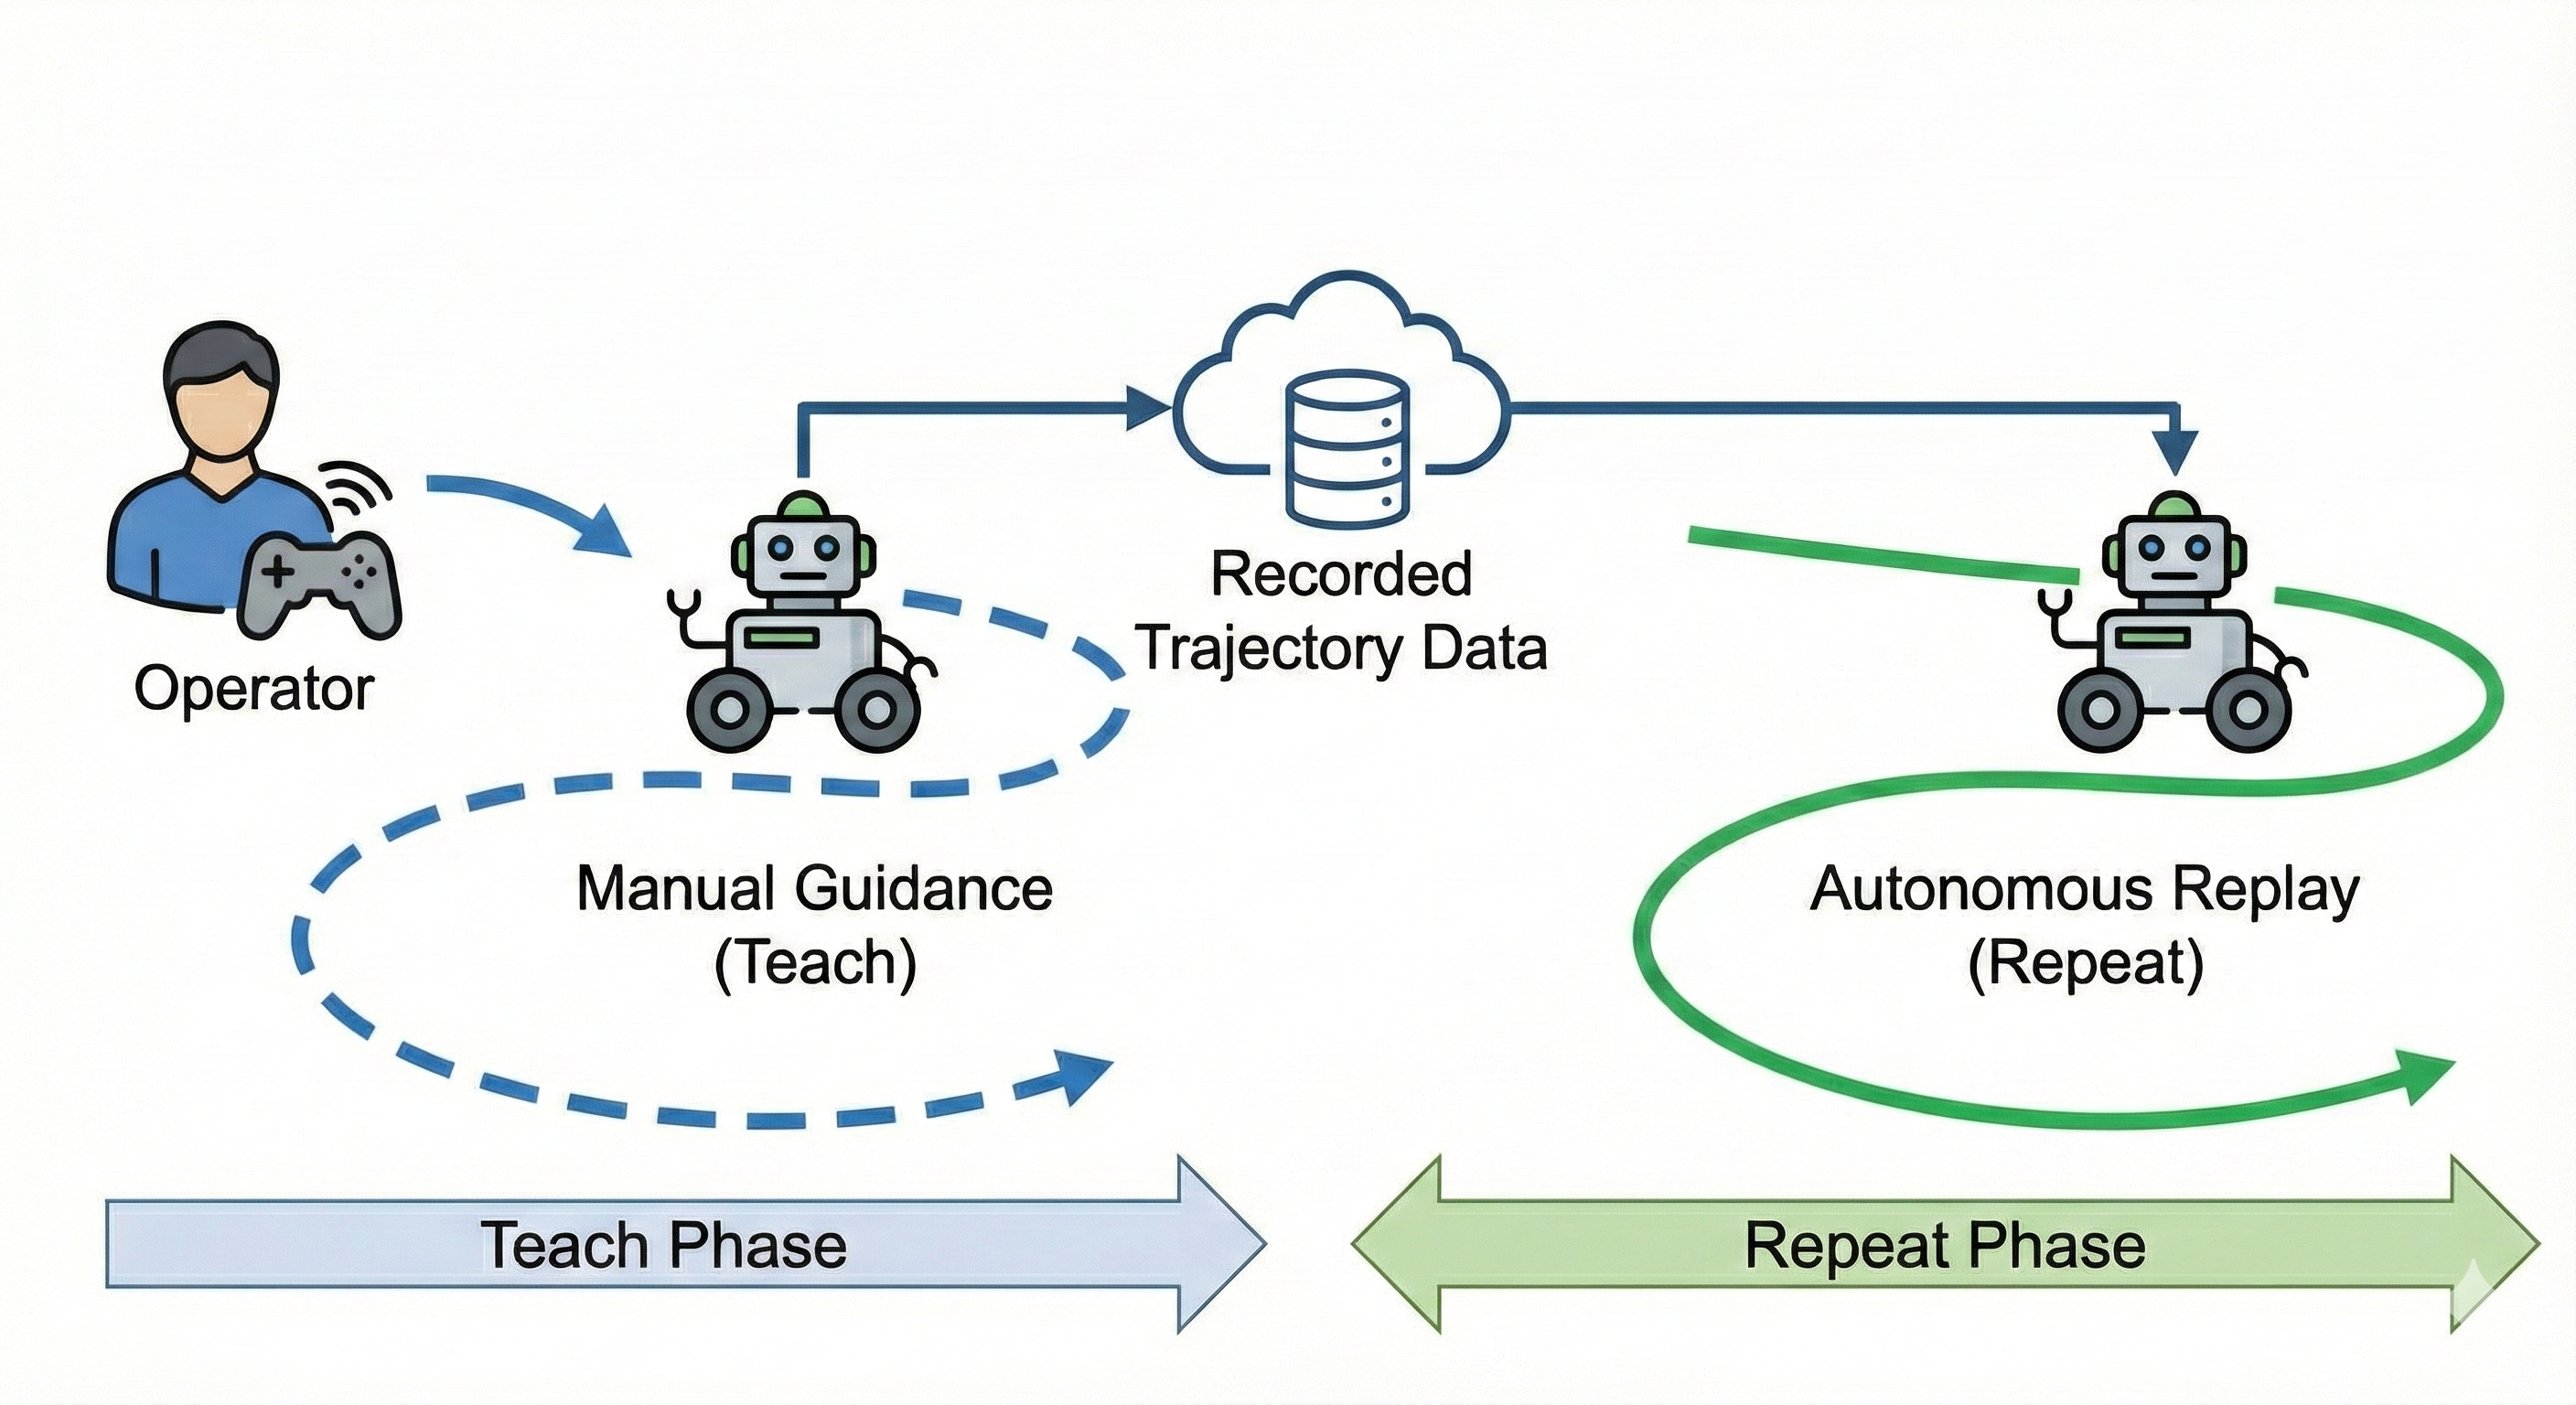
\includegraphics[trim={0.1cm 5cm 0.1cm 0.1cm}, clip, width=\textwidth]{assets/record_replay.png}\\[0.2cm]
				{\tiny\textit{Fig.3 — High-level teach and repeat concept}}
			}
		\end{column}
		
	\end{columns}
\end{frame}



% ==================/// PHASES ///==================
\section{Phases }
% ==================/// PHASE 1 ///==================
\begin{frame}{Phase 1: TF setup and perception}
    \begin{columns}[T]

        % LEFT: one step visible at a time
        \begin{column}{0.6\textwidth}
            {\small

            \only<1>{
                \textbf{Step 1 — Put tags on the map.}\\[0.2cm]
                We save where each AprilTag sits:
                \[
                    T_{\text{world}}^{\text{tag}}
                \]
                This stays fixed for every next step.
            }

            \only<2>{
                \textbf{Step 2 — Drive the robot once.}\\[0.2cm]
                The simulator gives the robot pose while it follows a smooth curve:
                \[
                    T_{\text{world}}^{\text{camera\_link}}(t)
                \]
            }

            \only<3>{
                \textbf{Step 3 — Use the real camera frame.}\\[0.2cm]
                We switch to the optical frame (how the camera really looks):
                \[
                    T_{\text{world}}^{\text{camera\_optical}}(t)
                    =
                    T_{\text{world}}^{\text{camera\_link}}(t)
                    \cdot
                    T_{\text{camera\_link}}^{\text{camera\_optical}}
                \]
            }

            \only<4>{
                \textbf{Step 4 — Compute clean tag detections.}\\[0.2cm]
                From the map and pose we get, for each tag:
                \[
                    T_{\text{camera\_optical}}^{\text{tag}}(t)
                \]
                This is the clean data that Phase 2 will dirty with noise.
            }

            }
        \end{column}

        % RIGHT: image appears from step 2 onwards and stays
        \begin{column}{0.35\textwidth}
            \centering
            \only<2->{
                \includegraphics[width=\textwidth]{assets/TF.png}
                \vspace{0.15cm}

                {\tiny\textit{Fig. 4 — World, robot and camera frames}}
            }
        \end{column}

    \end{columns}
\end{frame}



% ==================/// PHASE 2 ///==================
\begin{frame}{Phase 2: Simulation and dataset generation}
	\begin{columns}[T]
		
		% LEFT COLUMN
		\begin{column}{0.58\textwidth}
			\small
			
			\only<1>{
				\textbf{Step 1 — Simulate a clean path.}\\[0.2cm]
				We make a smooth curve and log the true pose:\\[0.1cm]
				\[
				T_{\text{world}}^{\text{camera\_optical}}(t)
				\]
			}
			
			\only<2>{
				\textbf{Step 2 — Compute perfect tag reads.}\\[0.2cm]
				For every tag and time we compute the clean detection:\\[0.1cm]
				\[
				T_{\text{camera\_optical}}^{\text{tag}}(t)
				\]
			}
			
			\only<3>{
				\textbf{Step 3 — Add noise like real life.}\\[0.2cm]
				We add Gaussian noise so readings look imperfect, like sensors do.
			}
			
			\only<4->{
				\textbf{Step 4 — Save the dataset.}\\[0.2cm]
				For each time we save:\\[0.1cm]
				- the true pose $T_{\text{world}}^{\text{camera\_optical}}(t)$\\
				- the noisy tag detections $T_{\text{camera\_optical}}^{\text{tag}}(t)$\\[0.2cm]
				Phase 3 will test its optimizer on this file.
			}
			
		\end{column}
		
		% RIGHT COLUMN — KEEP BIG IMAGES
		\begin{column}{0.40\textwidth}
			\centering
			
			\begin{overlayarea}{\textwidth}{0.60\textheight}
				
				% CLEAN IMAGE (large)
				\only<1>{
					\includegraphics[width=\textwidth]{assets/s_curve_dataset_large_plot_big.png}\\
					{\tiny\textit{Fig. 5 — Ground truth sinusoid trajectory}}
				}
				
				% NOISY IMAGE (large)
				\only<2>{
					\includegraphics[width=\textwidth]{assets/s_curve_dataset_large_noisy_plot_big.png}\\
					{\tiny\textit{Fig. 6 — Noisy measurements}}
				}
				
				% TWO BIG IMAGES STACKED (one above the other)
				\only<3->{
					\includegraphics[width=0.6\textwidth]{assets/s_curve_dataset_large_plot_big.png}\\[0.2cm]
					\includegraphics[width=0.6\textwidth]{assets/s_curve_dataset_large_noisy_plot_big.png}
					
					{\tiny\textit{Clean (top) and noisy (bottom) simulated data}}
				}
				
			\end{overlayarea}
		\end{column}
		
	\end{columns}
\end{frame}




% ==================/// PHASE 3 ///==================
\begin{frame}{Phase 3: Trajectory Optimization \& Recovery}
            \textbf{Goal: Fix drift with a simple optimizer}
            \vspace{0.5cm}
            \begin{itemize}
                \item<1-> \textbf{Path recovery:}  
                Align the noisy run with the taught path.

                \item<2-> \textbf{Pose graph:}  
                Reduce error between waypoints and simple constraints.

                \item<3-> \textbf{Drift fix:}  
                Auto-correct rotation and position drift.
            \end{itemize}
\end{frame}









\begin{frame}{Recovery the Optimal Path Sinusoidal Trajectory} % <-- Título mantido
    \centering
    \begin{columns}
        

        \begin{column}{0.5\textwidth}
            \centering
            % Sua imagem de recuperação
            \includegraphics[width=\textwidth]{assets/s_final_graph.png}
            \vspace{0.2cm}
            {\small\textit{Fig. 7.2 — Trajectory Recovery via Optimization}}
        \end{column}

        % COLUNA ESQUERDA: Dados Ruidosos
        \begin{column}{0.5\textwidth}
            \centering
            % Imagem do dataset ruidoso da Phase 2
            \includegraphics[width=\textwidth]{assets/slam_final__noise_graph.png}
            \vspace{0.2cm}
            {\small\textit{Fig. 7.1 — Simulated Dataset with Gaussian Noise}}
        \end{column}
        
        % COLUNA DIREITA: Caminho Otimizado/Recuperado
        
    \end{columns}
\end{frame}


\begin{frame}{Quantitative Analysis Sinusoidal Trajectory}
    \centering
    \footnotesize % Usa fonte um pouco menor para caber na coluna

    \begin{columns}[T] % Alinha o topo das colunas

        % ===================================
        % COLUNA 1: DADOS OTIMIZADOS SEM RUÍDO (Ideal - s_curve_otmires.png)
        % ===================================
        \begin{column}{0.48\textwidth}
            \centering
            \textbf{Case 1: Optimization without NOISE (Ideal)}
            \vspace{0.1cm}

            % Título principal dos resultados
            \begin{tabular}{lr}
                \toprule
                \textbf{Metric} & \textbf{Value} \\
                \midrule
                \textbf{Trajectory RMSE} & $\mathbf{0.0000 \text{ m}}$ \\ % Destacando o RMSE ideal
                Avg. Tag Position Error & $0.0164 \text{ m}$ \\
                \bottomrule
            \end{tabular}

            \vspace{0.3cm}
            
            % Tabela de Erro de Posição das AprilTags
            \textbf{Tag Estimation Error (Ideal)}
            \begin{tabular}{lccc}
                \toprule
                \textbf{Tag Name} & $\mathbf{X}$ \textbf{Error} & $\mathbf{Y}$ \textbf{Error} & $\mathbf{Z}$ \textbf{Error} \\
                \midrule
                tag36h11:0 & $0.00$ & $0.00$ & $0.00$ \\
                tag36h11:1 & $0.00$ & $0.00$ & $0.00$ \\
                tag36h11:2 & $0.01$ & $-0.01$ & $0.00$ \\
                tag36h11:3 & $0.03$ & $0.00$ & $0.00$ \\
                tag36h11:4 & $0.02$ & $-0.02$ & $0.00$ \\
                \bottomrule
            \end{tabular}
        \end{column}

        % LINHA VERTICAL (Opcional, para separar visualmente)
        \vrule width 0.1pt

        % ===================================
        % COLUNA 2: DADOS OTIMIZADOS COM RUÍDO (s_curve_noisy_otmires.png)
        % ===================================
        \begin{column}{0.48\textwidth}
            \centering
            \textbf{Case 2: Optimization with NOISE (6 cm)}
            \vspace{0.1cm}
            
            % Título principal dos resultados
            \begin{tabular}{lr}
                \toprule
                \textbf{Metric} & \textbf{Value} \\
                \midrule
                \textbf{Trajectory RMSE} & $\mathbf{0.0007 \text{ m}}$ \\ % Destacando o RMSE com ruído
                Avg. Tag Position Error & $0.0239 \text{ m}$ \\
                \bottomrule
            \end{tabular}

            \vspace{0.3cm}
            
            % Tabela de Erro de Posição das AprilTags
            \textbf{Tag Estimation Error}
            \begin{tabular}{lccc}
                \toprule
                \textbf{Tag Name} & $\mathbf{X}$ \textbf{Error} & $\mathbf{Y}$ \textbf{Error} & $\mathbf{Z}$ \textbf{Error} \\
                \midrule
                tag36h11:0 & $0.00$ & $0.01$ & $0.01$ \\
                tag36h11:1 & $0.01$ & $0.00$ & $0.00$ \\
                tag36h11:2 & $0.00$ & $-0.04$ & $0.01$ \\
                tag36h11:3 & $-0.01$ & $0.07$ & $0.00$ \\
                tag36h11:4 & $0.00$ & $-0.01$ & $0.00$ \\
                \bottomrule
            \end{tabular}
            
        \end{column}

    \end{columns}
    
    % LEGENDA FINAL
    \begin{center}
        \textit{Tables — Comparison of Optimization Results with and without noise.}
    \end{center}
\end{frame}



\begin{frame}{Recovery the Optimal Path Sinusoidal Trajectory}
    \centering
    
    % Título da seção (acima das colunas)
    \textbf{The scenario with 23 tags}
    \vspace{0.5cm}
    
    \begin{columns}
        
        % COLUNA 1 (ESQUERDA): Trajetória Recuperada (Recovery)
        \begin{column}{0.5\textwidth}
            \centering
            % Sua imagem de recuperação
            \includegraphics[width=\textwidth]{assets/s_20tags_final_graph.png}
            \vspace{0.2cm}
            {\small\textit{Fig. 8.1 — Trajectory Recovery via Optimization}} % Renomeei para 8.1 para manter a ordem lógica na tela
        \end{column}

        % COLUNA 2 (DIREITA): Dataset Ruidoso (Noisy Data)
        \begin{column}{0.5\textwidth}
            \centering
            % Imagem do dataset ruidoso da Phase 2
            \includegraphics[width=\textwidth]{assets/s_20tags_noise_final_graph.png}
            \vspace{0.2cm}
            {\small\textit{Fig. 8.2 — Simulated Dataset with Gaussian Noise}} % Renomeei para 8.2
        \end{column}
        
    \end{columns}
\end{frame}

\begin{frame}{Quantitative Analysis Sinusoidal Trajectory }
    \centering
    \footnotesize % Usa fonte um pouco menor para caber na coluna

    \centering
    
    % Título da seção (acima das colunas)
    \textbf{The scenario with 23 tags}
    \vspace{0.5cm}

    \begin{columns}[T] % Alinha o topo das colunas

        % ===================================
        % COLUNA 1: DADOS OTIMIZADOS SEM RUÍDO (Ideal - s_20tags_curve_otmires.png)
        % ===================================
        \begin{column}{0.48\textwidth}
            \centering
            \textbf{Case 1: Optimization without NOISE} 
            \vspace{0.1cm}

            % Tabela de Métricas (Mantida)
            \begin{tabular}{lr}
                \toprule
                \textbf{Metric} & \textbf{Value} \\
                \midrule
                \textbf{Trajectory RMSE} & $\mathbf{0.0002 \text{ m}}$ \\ 
                Avg. Tag Position Error & $0.0019 \text{ m}$ \\
                \bottomrule
            \end{tabular}

            \vspace{0.3cm}
            
            % Tabela de Erro de Posição das AprilTags (AMOSTRA)
            \textbf{Tag Estimation Error (Sample)}
            \begin{tabular}{lccc}
                \toprule
                \textbf{Tag Name} & $\mathbf{X}$ \textbf{Error} & $\mathbf{Y}$ \textbf{Error} & $\mathbf{Z}$ \textbf{Error} \\
                \midrule
                tag36h11:2 & $0.00$ & $0.00$ & $0.00$ \\
                tag36h11:7 & $0.00$ & $0.00$ & $0.00$ \\
                tag36h11:13 & $0.00$ & $0.00$ & $0.00$ \\
                tag36h11:18 & $0.00$ & $0.00$ & $0.00$ \\
                tag36h11:21 & $0.00$ & $0.00$ & $0.00$ \\
                \bottomrule
            \end{tabular}
        \end{column}

        % LINHA VERTICAL
        \vrule width 0.1pt

        % ===================================
        % COLUNA 2: DADOS OTIMIZADOS COM RUÍDO (s_20tags_curve_noisy_otmires.png)
        % ===================================
        \begin{column}{0.48\textwidth}
            \centering
            \textbf{Case 2: Optimization with NOISE (6 cm)} 
            \vspace{0.1cm}
            
            % Tabela de Métricas (Mantida)
            \begin{tabular}{lr}
                \toprule
                \textbf{Metric} & \textbf{Value} \\
                \midrule
                \textbf{Trajectory RMSE} & $\mathbf{0.0037 \text{ m}}$ \\ 
                Avg. Tag Position Error & $0.0134 \text{ m}$ \\
                \bottomrule
            \end{tabular}

            \vspace{0.3cm}
            
            % Tabela de Erro de Posição das AprilTags (AMOSTRA)
            \textbf{Tag Estimation Error (Sample)}
            \begin{tabular}{lccc}
                \toprule
                \textbf{Tag Name} & $\mathbf{X}$ \textbf{Error} & $\mathbf{Y}$ \textbf{Error} & $\mathbf{Z}$ \textbf{Error} \\
                \midrule
                tag36h11:2 & $0.01$ & $0.01$ & $0.00$ \\
                tag36h11:7 & $0.00$ & $0.00$ & $0.00$ \\
                tag36h11:13 & $0.01$ & $0.01$ & $0.00$ \\
                tag36h11:18 & $0.00$ & $0.00$ & $0.01$ \\
                tag36h11:21 & $0.01$ & $0.00$ & $0.02$ \\
                \bottomrule
            \end{tabular}
            
        \end{column}

    \end{columns}
    
    % LEGENDA FINAL
    \begin{center}
        \textit{Tables — Comparison of Optimization Results with and without noise (Sample of 5 Tags).}
    \end{center}
\end{frame}

\begin{frame}{Recovery the Optimal Path: Straight Trajectory}
    \centering
    
    \begin{columns}
        
        % COLUMN 1 (LEFT): Trajectory Recovery (Optimized)
        \begin{column}{0.5\textwidth}
            \centering
            % Assuming image name for the optimized straight trajectory
            \includegraphics[width=\textwidth]{assets/straight_final_graph.png}
            \vspace{0.2cm}
            {\small\textit{Fig. 8.1 — Trajectory Recovery via Optimization}} 
        \end{column}

        % COLUMN 2 (RIGHT): Noisy Dataset
        \begin{column}{0.5\textwidth}
            \centering
            % Assuming image name for the noisy straight trajectory dataset
            \includegraphics[width=\textwidth]{assets/straight_noisy_final_graph.png}
            \vspace{0.2cm}
            {\small\textit{Fig. 8.2 — Simulated Dataset with Gaussian Noise}} 
        \end{column}
        
    \end{columns}
\end{frame}

\begin{comment}


\begin{frame}{Quantitative Analysis: Straight Trajectory}
    \centering
    \footnotesize % Use smaller font size to fit content

    \begin{columns}[T] % Align the top of the columns

        % ===================================
        % COLUMN 1: DATA WITHOUT NOISE (IDEAL)
        % ===================================
        \begin{column}{0.48\textwidth}
            \centering
            {\tiny (Data Source: straight\_otmires.png)}
            \vspace{0.1cm}
            
            \textbf{Case 1: Optimization without NOISE}
            \vspace{0.1cm}

            % Metrics Table
            \begin{tabular}{lr}
                \toprule
                \textbf{Metric} & \textbf{Value} \\
                \midrule
                \textbf{Trajectory RMSE} & $\mathbf{0.0017 \text{ m}}$ \\
                Avg. Tag Position Error & $\mathbf{0.0000 \text{ m}}$ \\
                \bottomrule
            \end{tabular}

            \vspace{0.3cm}
            
            % Tag Estimation Error Table
            \textbf{Tag Estimation Error (Ideal)}
            \begin{tabular}{lc}
                \toprule
                \textbf{Tag Name} & \textbf{Error (m)} \\
                \midrule
                tag36h11:1 & $0.0000$ \\
                tag36h11:2 & $0.0000$ \\
                tag36h11:3 & $0.0000$ \\
                tag36h11:4 & $0.0000$ \\
                tag36h11:5 & $0.0000$ \\
                tag36h11:6 & $0.0000$ \\
                \bottomrule
            \end{tabular}
        \end{column}

        % VERTICAL LINE
        \vrule width 0.1pt

        % ===================================
        % COLUMN 2: DATA WITH NOISE
        % ===================================
        \begin{column}{0.48\textwidth}
            \centering
            {\tiny (Data Source: straight\_noisy\_otmires.png)}
            \vspace{0.1cm}
            
            \textbf{Case 2: Optimization with NOISE}
            \vspace{0.1cm}
            
            % Metrics Table
            \begin{tabular}{lr}
                \toprule
                \textbf{Metric} & \textbf{Value} \\
                \midrule
                \textbf{Trajectory RMSE} & $\mathbf{0.0007 \text{ m}}$ \\
                Avg. Tag Position Error & $\mathbf{0.0248 \text{ m}}$ \\
                \bottomrule
            \end{tabular}

            \vspace{0.3cm}
            
            % Tag Estimation Error Table
            \textbf{Tag Estimation Error}
            \begin{tabular}{lc}
                \toprule
                \textbf{Tag Name} & \textbf{Error (m)} \\
                \midrule
                tag36h11:1 & $0.0115$ \\
                tag36h11:2 & $0.0337$ \\
                tag36h11:3 & $0.0363$ \\
                tag36h11:4 & $0.0288$ \\
                tag36h11:5 & $0.0139$ \\
                tag36h11:6 & $0.0245$ \\
                \bottomrule
            \end{tabular}
            
        \end{column}

    \end{columns}
    
    % FINAL CAPTION
    \begin{center}
        \textit{Comparison: Ideal Case vs. Noisy Case (Results from Python Optimization)}
    \end{center}
\end{frame}


% ==================/// PHASE 4 ///==================
\begin{frame}{Phase 4: Robot implementation}
    \begin{columns}[T] % [T] Alinha o conteúdo pelo topo
        
        % --- Coluna da Esquerda (Texto) ---
        \begin{column}{0.6\textwidth}
            \textbf{Goal: Move from PC tests to the LIMOS robot}
            \vspace{0.5cm}
            \begin{itemize}
                \setlength\itemsep{1em} % Espaçamento entre itens
                
                \item<1-> \textbf{Onboard integration:}  
                Put the perception code on the robot (ROS~2).

                \item<3-> \textbf{Camera calibration:}  
                Calibrate the camera so distances look right.

                \item<5-> \textbf{First trajectory recording:}  
                Record one path using wheels plus AprilTag pose.
            \end{itemize}
        \end{column}
        
        % --- Coluna da Direita (Imagens) ---
        \begin{column}{0.38\textwidth}
            \centering
            % overlayarea reserva o espaço para evitar que o slide pule na troca
            \begin{overlayarea}{\textwidth}{0.6\textheight}
                \centering
                
                % IMAGEM 1: Aparece no slide 2 e SOME no final do slide 3
                \only<2>{
                    \includegraphics[width=\textwidth, keepaspectratio]{assets/limo.jpeg}
                    \vspace{0cm}
                    \\{\tiny\textit{Fig. 8 — LIMOS platform}}
                }sinusoidal
                
                % IMAGEM 2: Aparece no slide 4 e fica até o fim
                % (Coloquei o mesmo nome de arquivo, mas idealmente seria outra foto)
                \only<4->{
                    \includegraphics[trim={5cm 3cm 5cm 2cm}, clip, width=\textwidth]{assets/camera_calibration.jpg}
                    \vspace{0cm}
                    \\{\tiny\textit{Fig. 9 — Calibration}}
                }
            \end{overlayarea}
        \end{column}
        
    \end{columns}
\end{frame}

\end{comment}


\begin{frame}{Quantitative Analysis: Straight Trajectory}
    \centering
    \footnotesize % Use smaller font size to fit content

    \centering
    


    \begin{columns}[T] % Align the top of the columns

        % ===================================
        % COLUMN 1: DATA WITHOUT NOISE
        % ===================================
        \begin{column}{0.48\textwidth}
            \centering
            % Texto da fonte

            \vspace{0.1cm}
            
            \textbf{Case 1: Optimization without NOISE}
            \vspace{0.1cm}

            % Metrics Table
            \begin{tabular}{lr}
                \toprule
                \textbf{Metric} & \textbf{Value} \\
                \midrule
                \textbf{Trajectory RMSE} & $\mathbf{0.0017 \text{ m}}$ \\
                Avg. Tag Position Error & $0.0000 \text{ m}$ \\
                \bottomrule
            \end{tabular}

            \vspace{0.3cm}
            
            % Tag Estimation Error Table
            \textbf{Tag Estimation Error (Sample)}
            \begin{tabular}{lccc}
                \toprule
                \textbf{Tag Name} & $\mathbf{X}$ \textbf{Error} & $\mathbf{Y}$ \textbf{Error} & $\mathbf{Z}$ \textbf{Error} \\
                \midrule
                tag36h11:0 & $0.00$ & $0.00$ & $0.00$ \\
                tag36h11:1 & $0.00$ & $0.00$ & $0.00$ \\
                tag36h11:2 & $0.00$ & $0.00$ & $0.00$ \\
                tag36h11:3 & $0.00$ & $0.00$ & $0.00$ \\
                tag36h11:4 & $0.00$ & $0.00$ & $0.00$ \\
                \bottomrule
            \end{tabular}
        \end{column}

        % VERTICAL LINE
        \vrule width 0.1pt

        % ===================================
        % COLUMN 2: DATA WITH NOISE
        % ===================================
        \begin{column}{0.48\textwidth}
            \centering
            % Texto da fonte
            \vspace{0.1cm}
            
            \textbf{Case 2: Optimization with NOISE (6 cm)}
            \vspace{0.1cm}
            
            % Metrics Table
            \begin{tabular}{lr}
                \toprule
                \textbf{Metric} & \textbf{Value} \\
                \midrule
                \textbf{Trajectory RMSE} & $\mathbf{0.017 \text{ m}}$ \\
                Avg. Tag Position Error & $0.01912 \text{ m}$ \\
                \bottomrule
            \end{tabular}

            \vspace{0.3cm}
            
            % Tag Estimation Error Table
            \textbf{Tag Estimation Error (Sample)}
            \begin{tabular}{lccc}
                \toprule
                \textbf{Tag Name} & $\mathbf{X}$ \textbf{Error} & $\mathbf{Y}$ \textbf{Error} & $\mathbf{Z}$ \textbf{Error} \\
                \midrule
                tag36h11:0 & $0.01$ & $0.01$ & $0.00$ \\
                tag36h11:1 & $0.00$ & $0.00$ & $0.00$ \\
                tag36h11:2 & $0.01$ & $0.01$ & $0.00$ \\
                tag36h11:3 & $0.00$ & $0.00$ & $0.01$ \\
                tag36h11:4 & $0.01$ & $0.00$ & $0.02$ \\
                \bottomrule
            \end{tabular}
            
        \end{column}

    \end{columns}
    
    % FINAL CAPTION
    \begin{center}
        \textit{Tables — Comparison of Optimization Results with and without noise (Sample of 5 Tags).}
    \end{center}
\end{frame}

% ==================/// PHASE 5 ///==================
\begin{frame}{Phase 5: Path recovery algorithm}
    \begin{columns}
        \begin{column}{0.6\textwidth}
            \textbf{Goal: Recover when the robot leaves the taught path}
            \vspace{0.5cm}
            \begin{itemize}
                \item<1-> \textbf{Recovery logic:}  
                Simple rules to steer back to the recorded path.

                \item<2-> \textbf{Closest waypoint search:}  
                Use a quick KD-Tree to find the nearest waypoint.

                \item<4-> \textbf{Safety validation:}  
                Test recovery moves in sim to avoid bad turns.
            \end{itemize}
        \end{column}
        
        \begin{column}{0.50\textwidth}
            \centering
            \only<3->{
                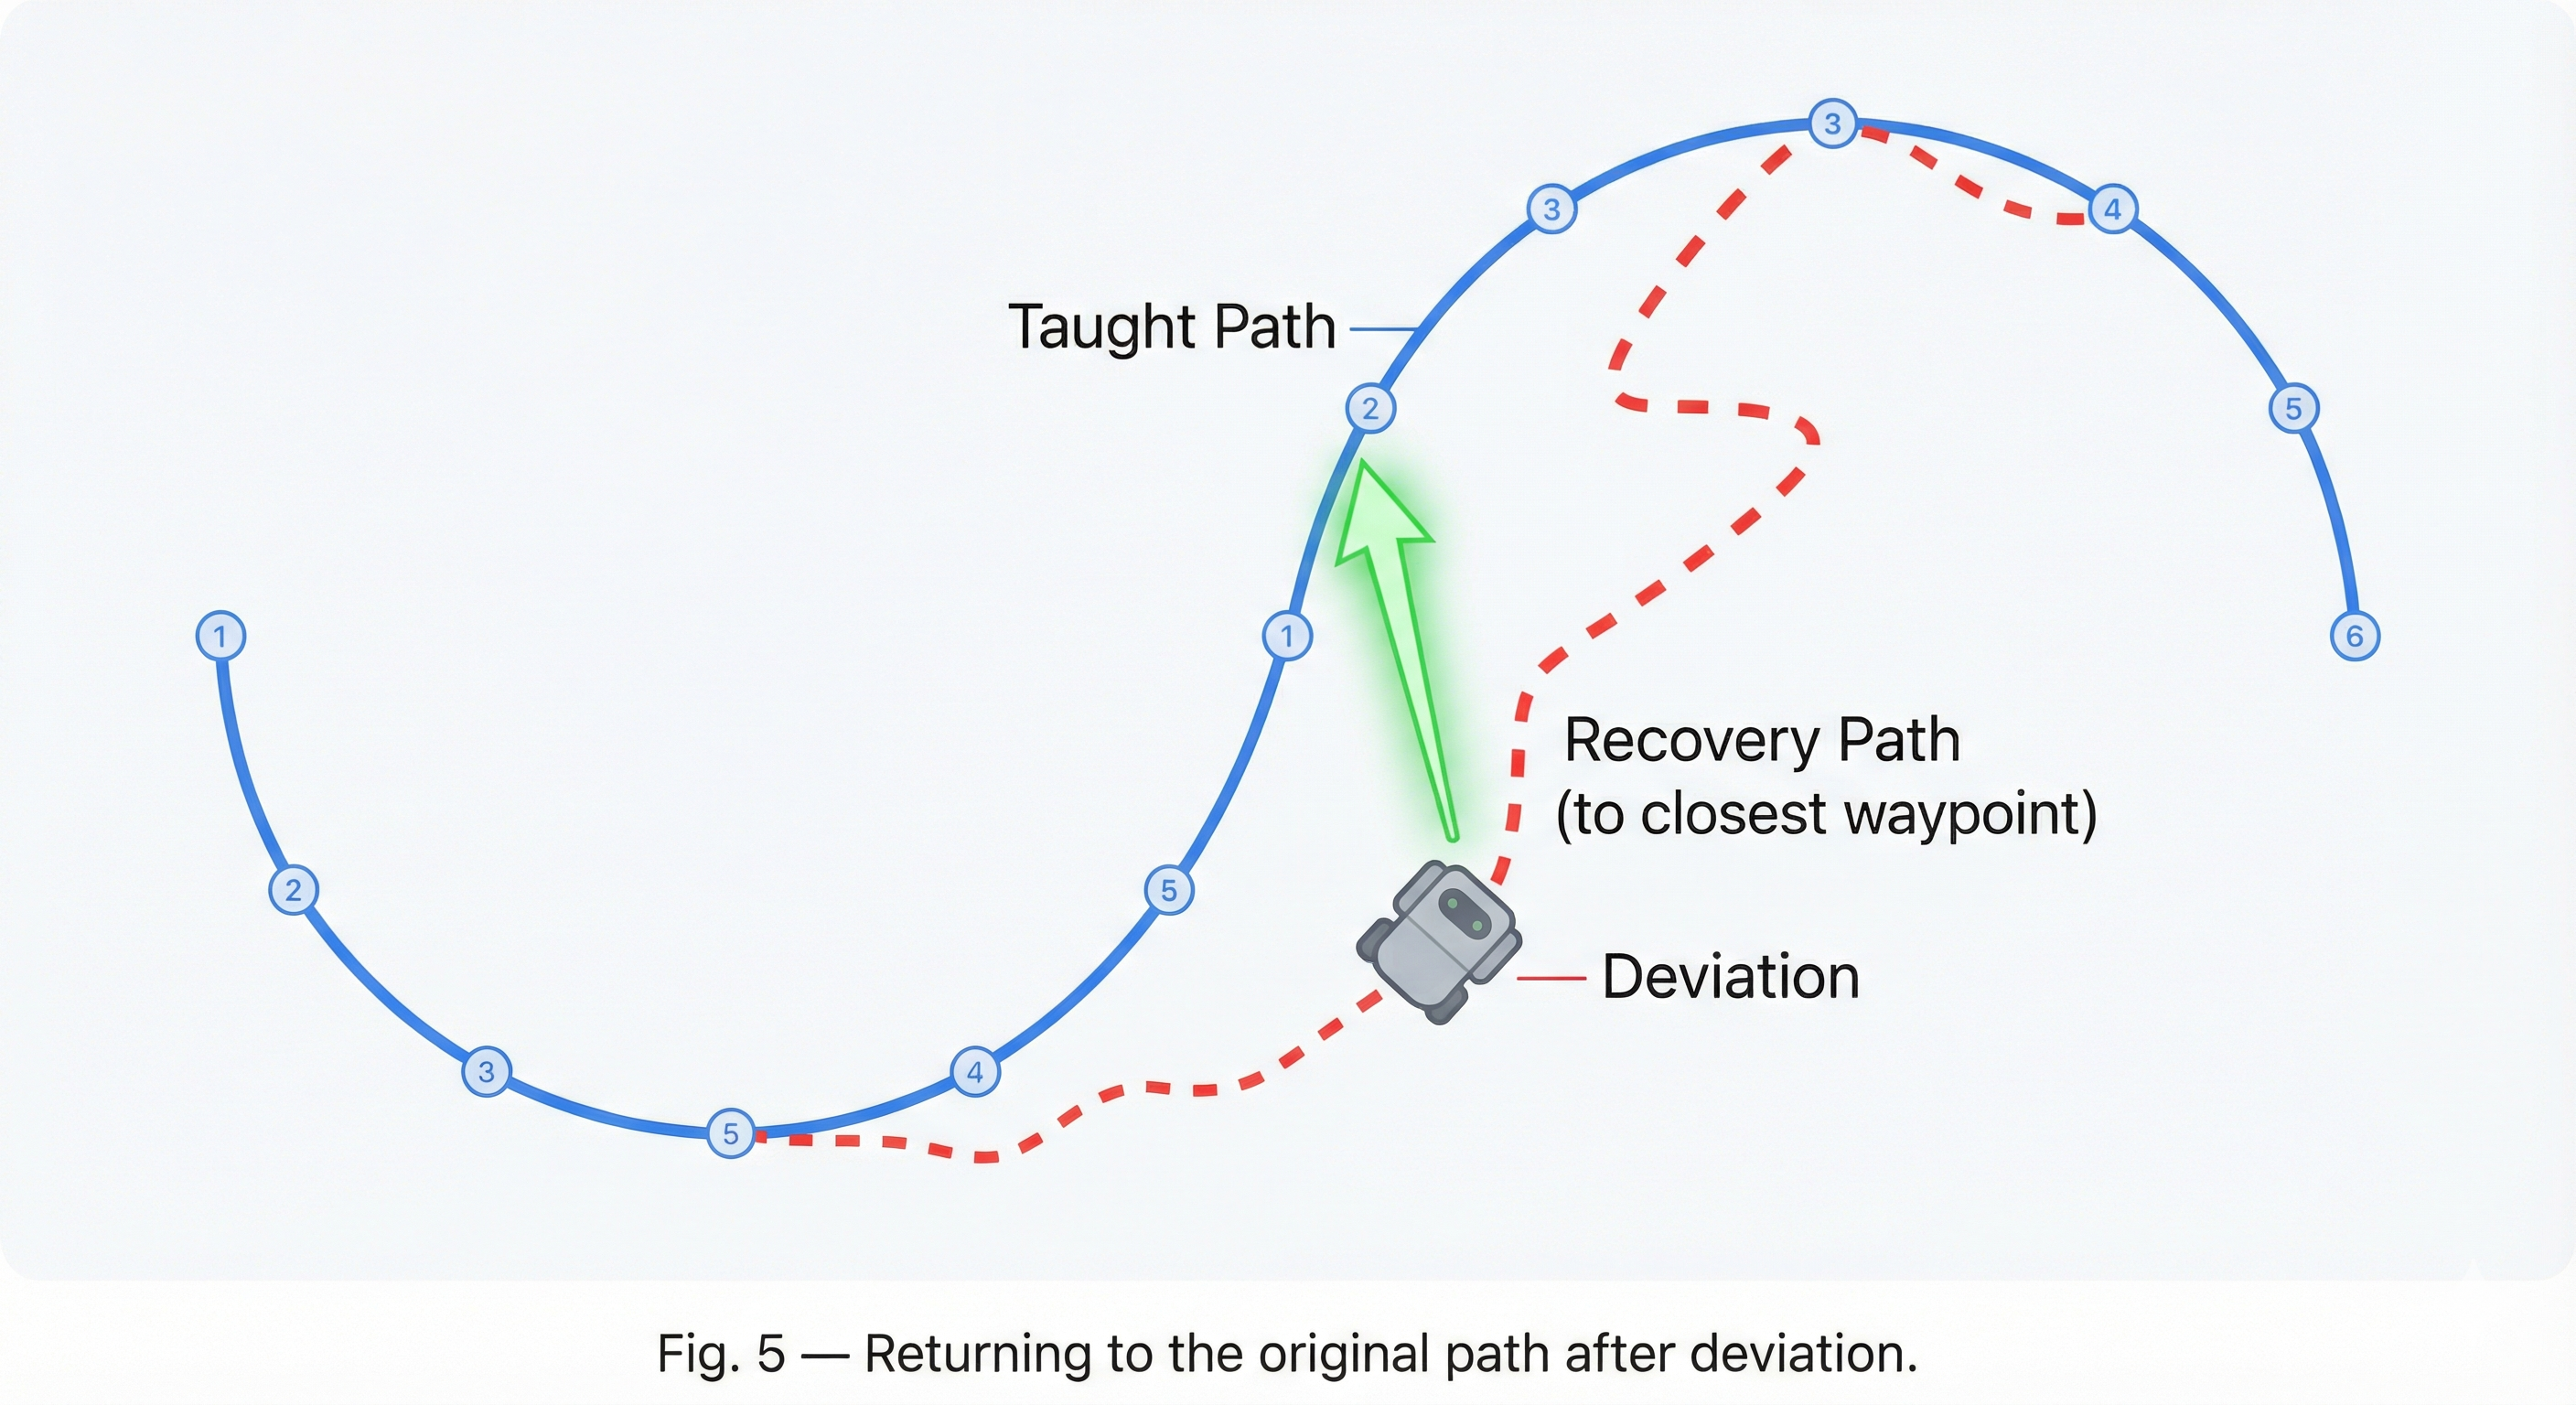
\includegraphics[trim={5cm 4cm 5cm 3cm}, clip, width=\textwidth]{assets/return_path.png}

                \vspace{0.2cm}
                {\tiny\textit{Fig. 10 — Returning to the original path after deviation}}
            }
        \end{column}
    \end{columns}
\end{frame}



% ==================/// PHASE 6 ///==================
\begin{frame}{Phase 6: System integration}
    \begin{columns}
        \begin{column}{0.6\textwidth}
            \textbf{Goal: Demonstrate full teach and repeat autonomy}
            \vspace{0.5cm}
            \begin{itemize}
                \item<1-> \textbf{Controller integration:}  
                Mix Pure Pursuit with the perception and pose stack.

                \item<2-> \textbf{Autonomous replay:}  
                Let the robot drive the recorded path on its own.

                \item<4-> \textbf{Final system:}  
                A teach \& repeat pipeline anyone can run without coding.
            \end{itemize}
        \end{column}
        
        \begin{column}{0.45\textwidth}
            \centering
            \only<3->{
                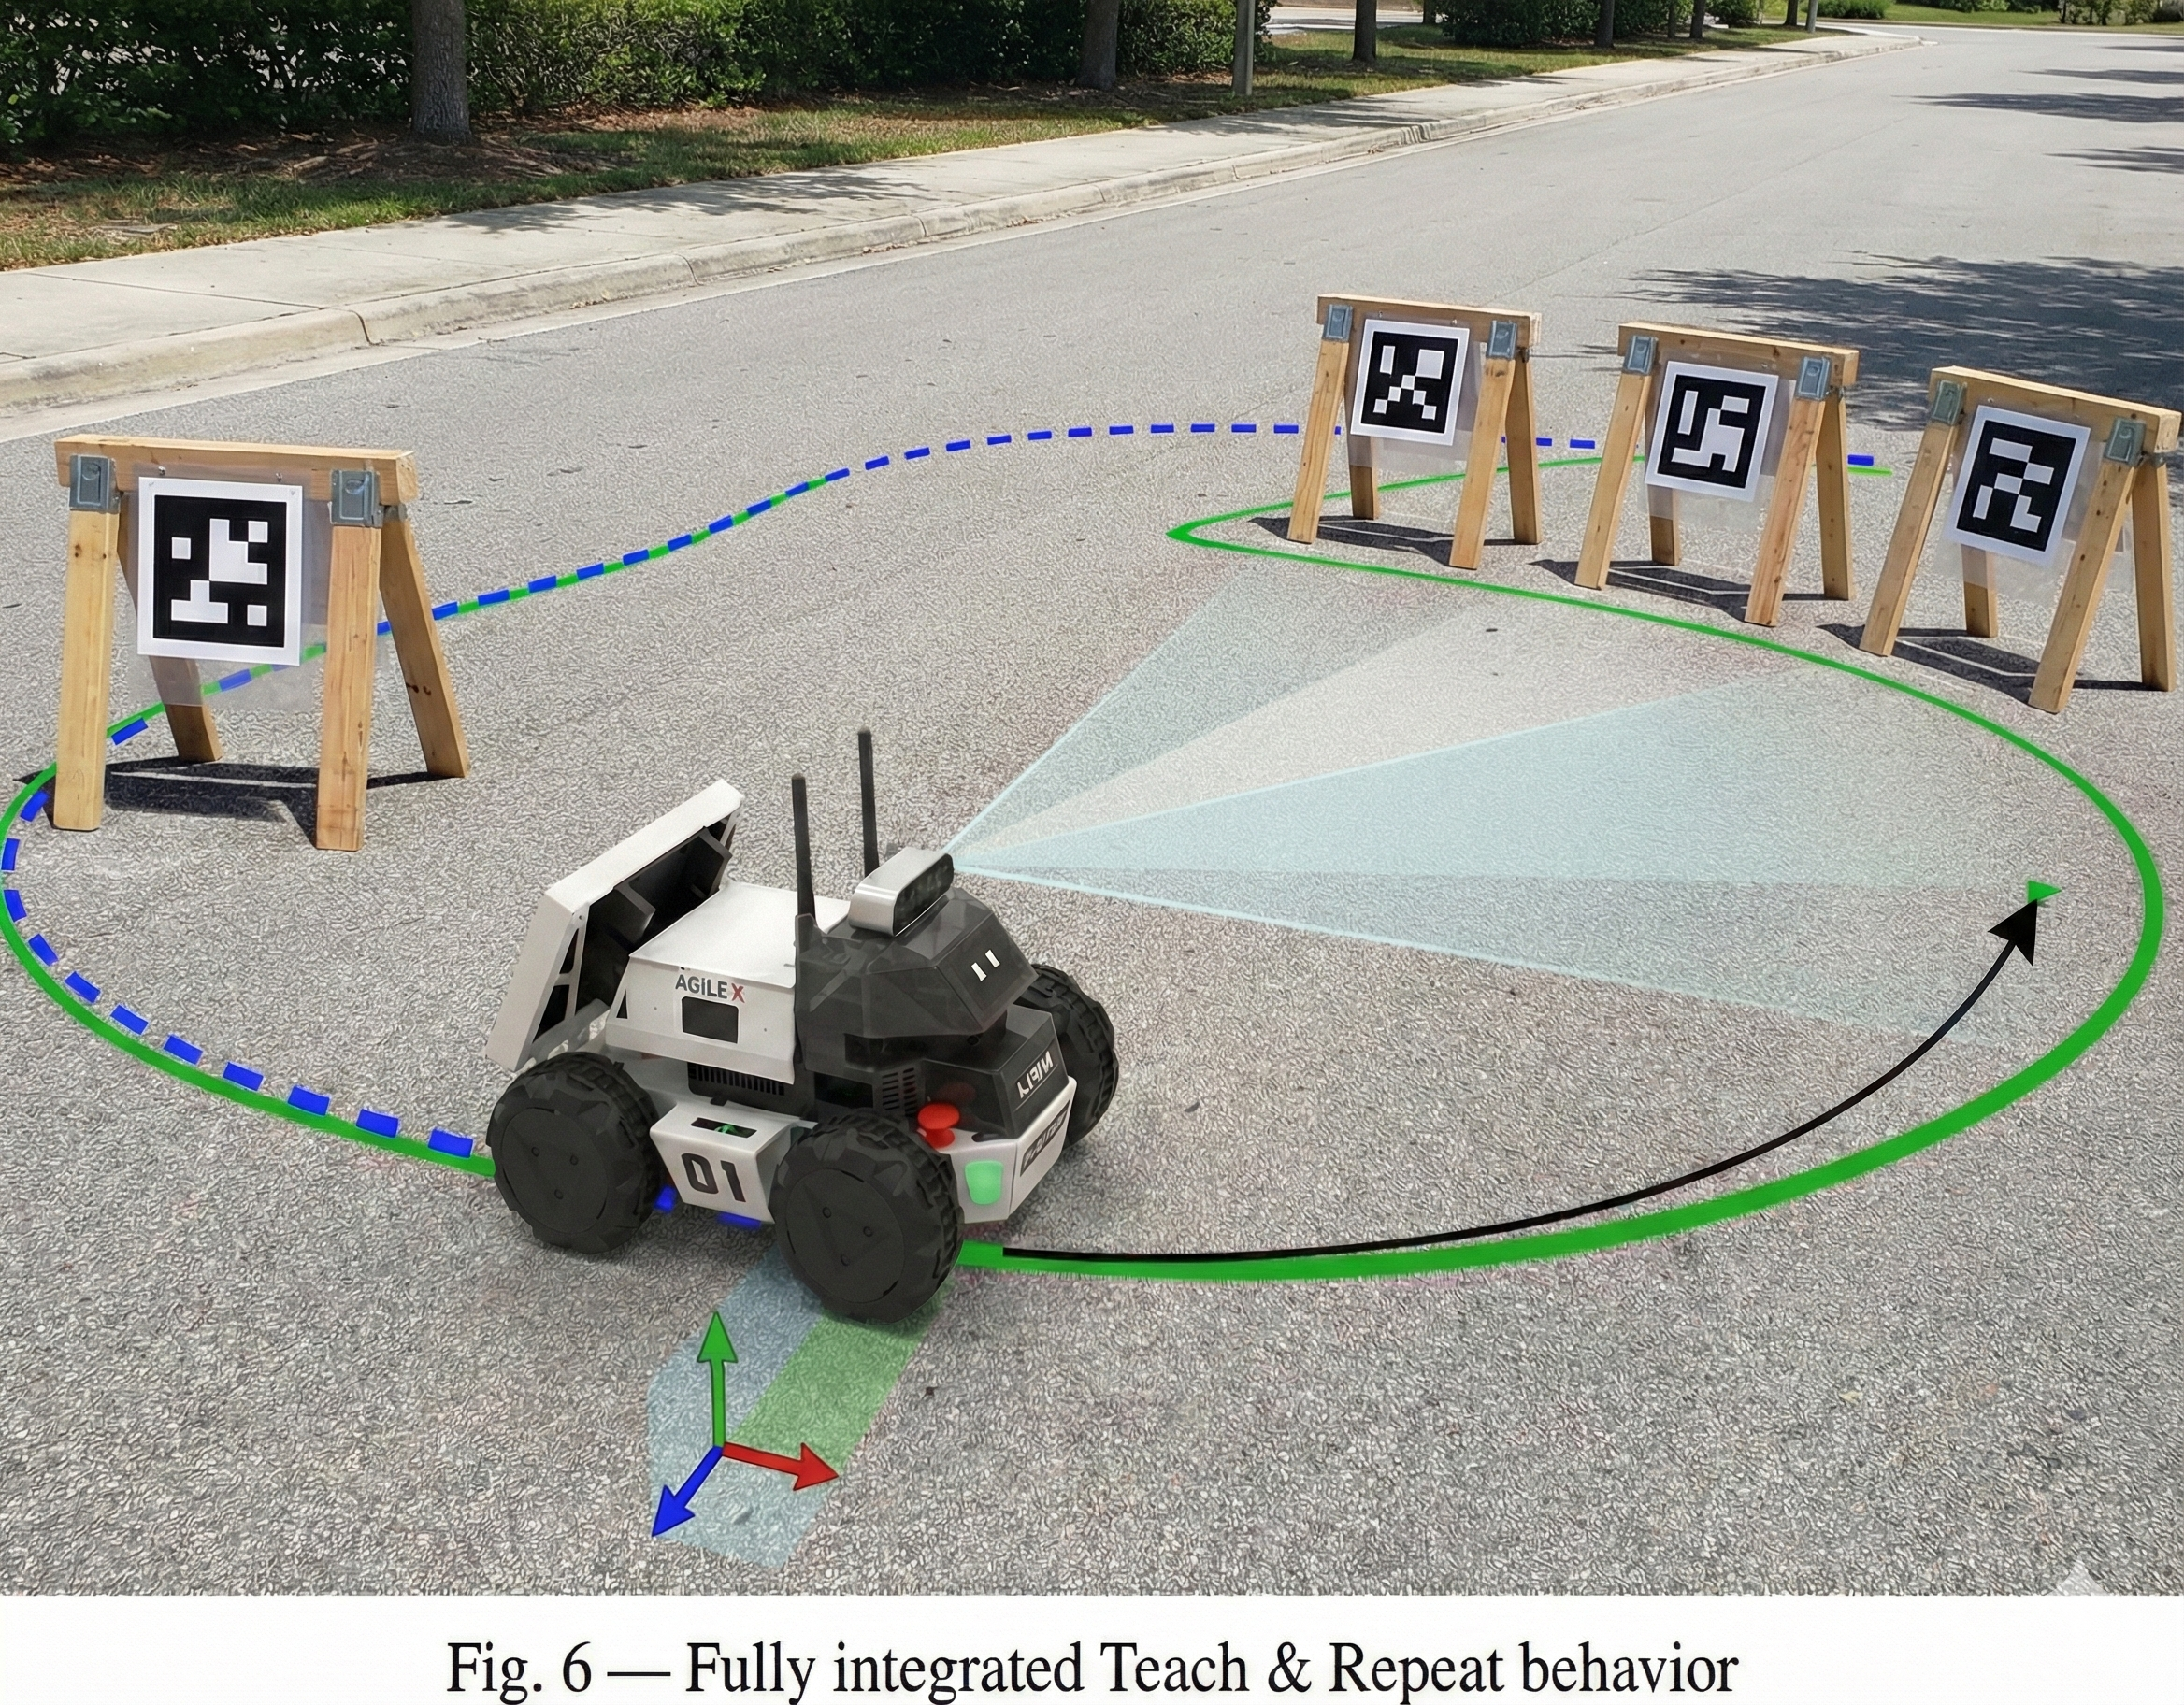
\includegraphics[trim={1cm 5cm 1cm 1cm}, clip, width=\textwidth]{assets/robot_transit.png}

                \vspace{0.2cm}
                {\tiny\textit{Fig. 11 — Fully integrated teach and repeat behavior}}
            }
        \end{column}
    \end{columns}
\end{frame}



\begin{frame}[allowframebreaks]{References}
    % Remove ícones e usa numeração [1]
    \setbeamertemplate{bibliography item}[text]
    
    % Fonte pequena
    \scriptsize 
    
    \begin{thebibliography}{99}
        
        \bibitem{adamek2023analytical}
        R.~Adámek, M.~Brablc, P.~Vávra, B.~Dobossy, M.~Formánek, and F.~Radil, ``Analytical Models for Pose Estimate Variance of Planar Fiducial Markers for Mobile Robot Localisation'', \emph{Sensors}, vol.~23, no.~12, p.~5746, 2023. DOI: \url{10.3390/s23125746}

        \bibitem{herrera2025visual}
        B.~S.~Herrera, M.~García, W.~Chamorro, and D.~Maldonado, ``Visual Mapping and Autonomous Navigation Using AprilTags in Omnidirectional Mobile Robots: A Realistic ROS-Gazebo Simulation Framework'', \emph{Engineering Proceedings}, vol.~115, no.~1, p.~5, 2025. DOI: \url{10.3390/engproc2025115005}

        \bibitem{thrun2005probabilistic}
        S.~Thrun, W.~Burgard, and D.~Fox, \emph{Probabilistic Robotics}, MIT Press, 2005. DOI: \url{10.5555/1625995.1626105}

        \bibitem{pfrommer2019tagslam}
        B.~Pfrommer and K.~Daniilidis, ``TagSLAM: Robust SLAM with Fiducial Markers'', \emph{arXiv preprint arXiv:1910.00679}, 2019. DOI: \url{10.48550/arXiv.1910.00679}

    \end{thebibliography}
\end{frame}


% ==================///==================///==================///
% ==================/// BODY'S PRESENTATION
% ==================///==================///==================///

\input{sections/introduction}

\input{sections/personalization}

\input{chapters/special_slides}


% ==================/// END PRESENTATION
% ==================///==================///==================///

\begin{frame}[plain]
	
	% Logos no canto superior direito (como nos outros slides)
	\begin{tikzpicture}[remember picture,overlay]
		\node[anchor=north east] 
		at ($(current page.north east)+(-0.8cm,-0.6cm)$) {
			\includegraphics[height=1.0cm]{assets/logo_UCA.jpg}

		};
	\end{tikzpicture}
	
	\centering
	\vspace*{2.2cm}
	
	{\Huge\bfseries\textcolor{NavyBlue}{Thank you for listening!}\par}
	\vspace{0.4cm}
	{\Large\textcolor{CoolGray}{Any questions?}\par}
	
	\vspace{0.9cm}
	{\color{AccentBlue}\rule{3cm}{1.5pt}\par}
	
	\vspace{0.7cm}
	{\small\textcolor{CoolGray}{ Joao Pedro Martins do Lago Reis \quad|\quad Yann Kelvem da Silva Ramos}\par}
	{\small\textcolor{CoolGray}{AprilTag-based Trajectory Tracking for the LIMOS Robot}\par}
	
\end{frame}


\end{document}
